
%\textcolor{red}{Why do we need a bank of hybrids?}\newline
The template bank contructed in Sec.~\ref{s1:NRonlybank} is effectual for 
GW detection searches focussed at relatively massive binaries with 
$\mathcal{M}_c \gtrsim 27M_\odot$. As the NR waveforms are restricted to a
small number of orbits, it is useful to consider NR-PN hybrids to bring the
lower mass limit down on the template bank. PN waveforms can be generated
for an arbitrarily large number of inspiral orbits, reasonably accurately and
relatively cheaply. Thus, a hybrid waveform comprised of a long PN early-inspiral 
and an NR late-inspiral, merger, and ringdown could also be arbitrarily long. 
There are, however, uncertainties in the PN waveforms, due to
the unknown higher-order terms. During the late-inspiral and merger phase,
these terms become more important and the PN description becomes
less accurate. In addition, when more of the late-inspiral is
in the detector's sensitivity frequency range, hybrid waveform mismatches 
due to the PN errors become increasingly large, and reduce the
recovered SNR. Thus, when
hybridizing PN and NR waveforms, there must be enough NR orbits that the PN
error is sufficiently low for the considered detector noise-curve. In 
this section, we construct an NR + PN hybrid template bank, for currently
available NR waveforms, and determine the lowest value of binary masses to 
which it covers.


%\subsubsection{Including hybrid PN error}\label{s2:HybridPNerror}
\begin{figure}
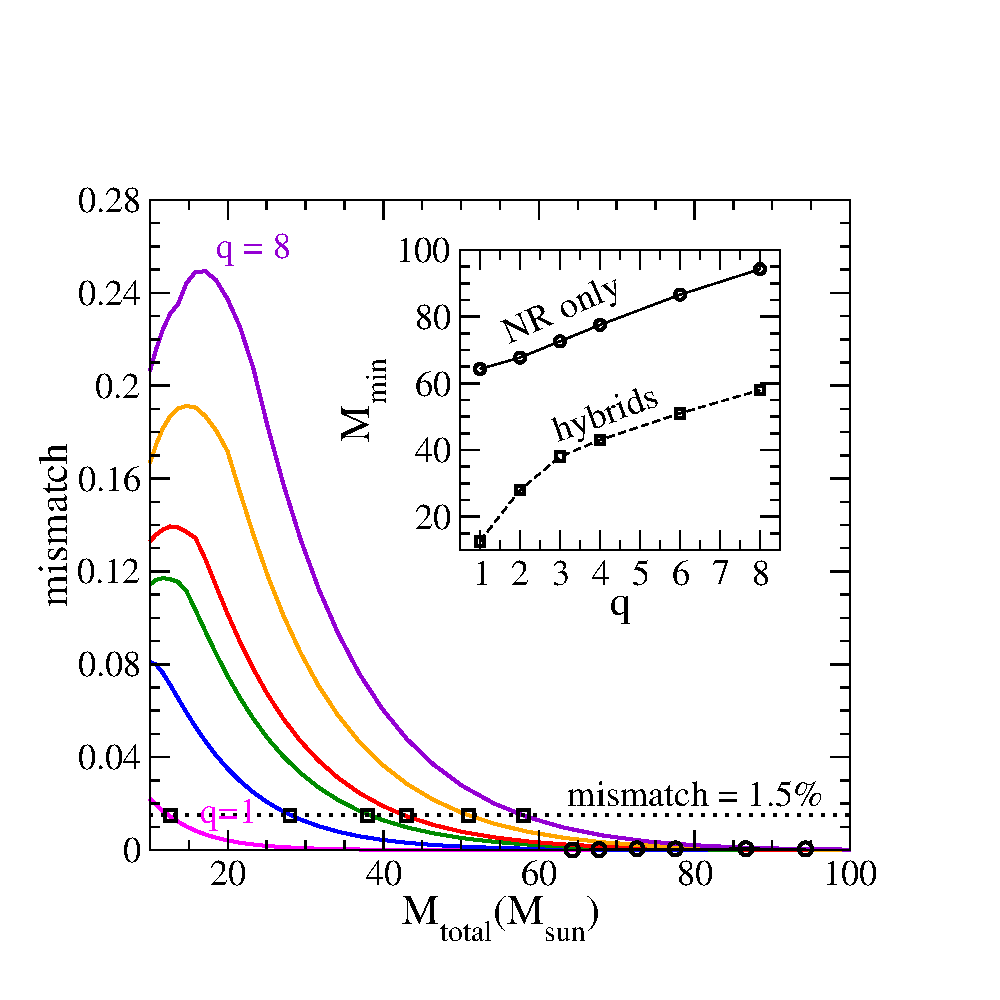
\includegraphics[width=0.9\columnwidth, trim=20 17 75 75]{maxmismatchVSmass_allq.pdf}
\caption{\label{fig:Current-NR-PN-Errors}Bounds on mismatches of PN-NR
  hybrid waveforms, for the currently existing NR simulations. The PN
  error is for hybrids matched at $M\omega_m=0.025$ for $q=1$,
  $M\omega_m=0.038$ for $q=2$, and $M\omega_m=0.042$ for
  $q=3,4,6,8$. The black circles indicate the lower bound of the
  template bank in Sec.~\ref{s1:NRonlybank}. The black square show the
  lower bound with a hybrid error of 1.5\%. The inset shows these
  lower bounds as a function of mass ratio.} 
\end{figure}

%\textcolor{red}{Details of hybrids and how we estimate their errors?}\newline
The hybrids we use are constructed by joining the PN and NR portions, as 
described in Sec.~\ref{s2:NRpNhybridwaveforms}. The number of orbits before 
merger at which they are joined depends on the length of the available NR 
waveforms. We estimate the PN waveform errors using hybridization
mismatches $\Gamma_\Hyb$, as discussed in Sec.~\ref{s1:quantifyingerrors}. 
Fig.~\ref{fig:Current-NR-PN-Errors} shows the same for all the hybrids, as a 
function of total mass. In terms of orbital frequency, these are
matched at $M\omega_m=0.025$ for $q=1$, $M\omega_m=0.038$ for $q=2$,
and $M\omega_m=0.042$ for $q=3,4,6,8$. In terms of number of orbits
before merger, this is 31.9 orbits for $q=1$, 17.8 orbits for $q=2$,
16.9 orbits for $q=3$, 18.4 orbits for $q=4$, 21.6 orbits for $q=6$,
and 25.1 orbits for $q=8$. The dotted line indicates a mismatch of
$1.5\%$, a comparatively tight bound that leaves flexibility to accommodate
errors due to template bank discreteness. The black circles show the hybrid
mismatches at the lower mass bound of the NR-only template bank in
Sec.~\ref{s1:NRonlybank}, which are negligible. The inset shows this minimum 
mass as a function of mass ratio, as well as the minimum attainable mass if we
accept a hybrid error of $1.5\%$. At lower masses, the mismatches increase
sharply with more of the PN part moving into the Advanced LIGO sensitivity band.
This is due to the nature of the frequency dependence of the detector 
sensitivity. The detectors will be relatively very sensitive to a relatively 
short frequency band. As the hybridization frequency sweeps through that band, 
the hybrid errors rise sharply. They fall again at the lowest masses, for which
mostly the PN portion stays within the sensitive band.


\begin{figure*}
\begin{center}
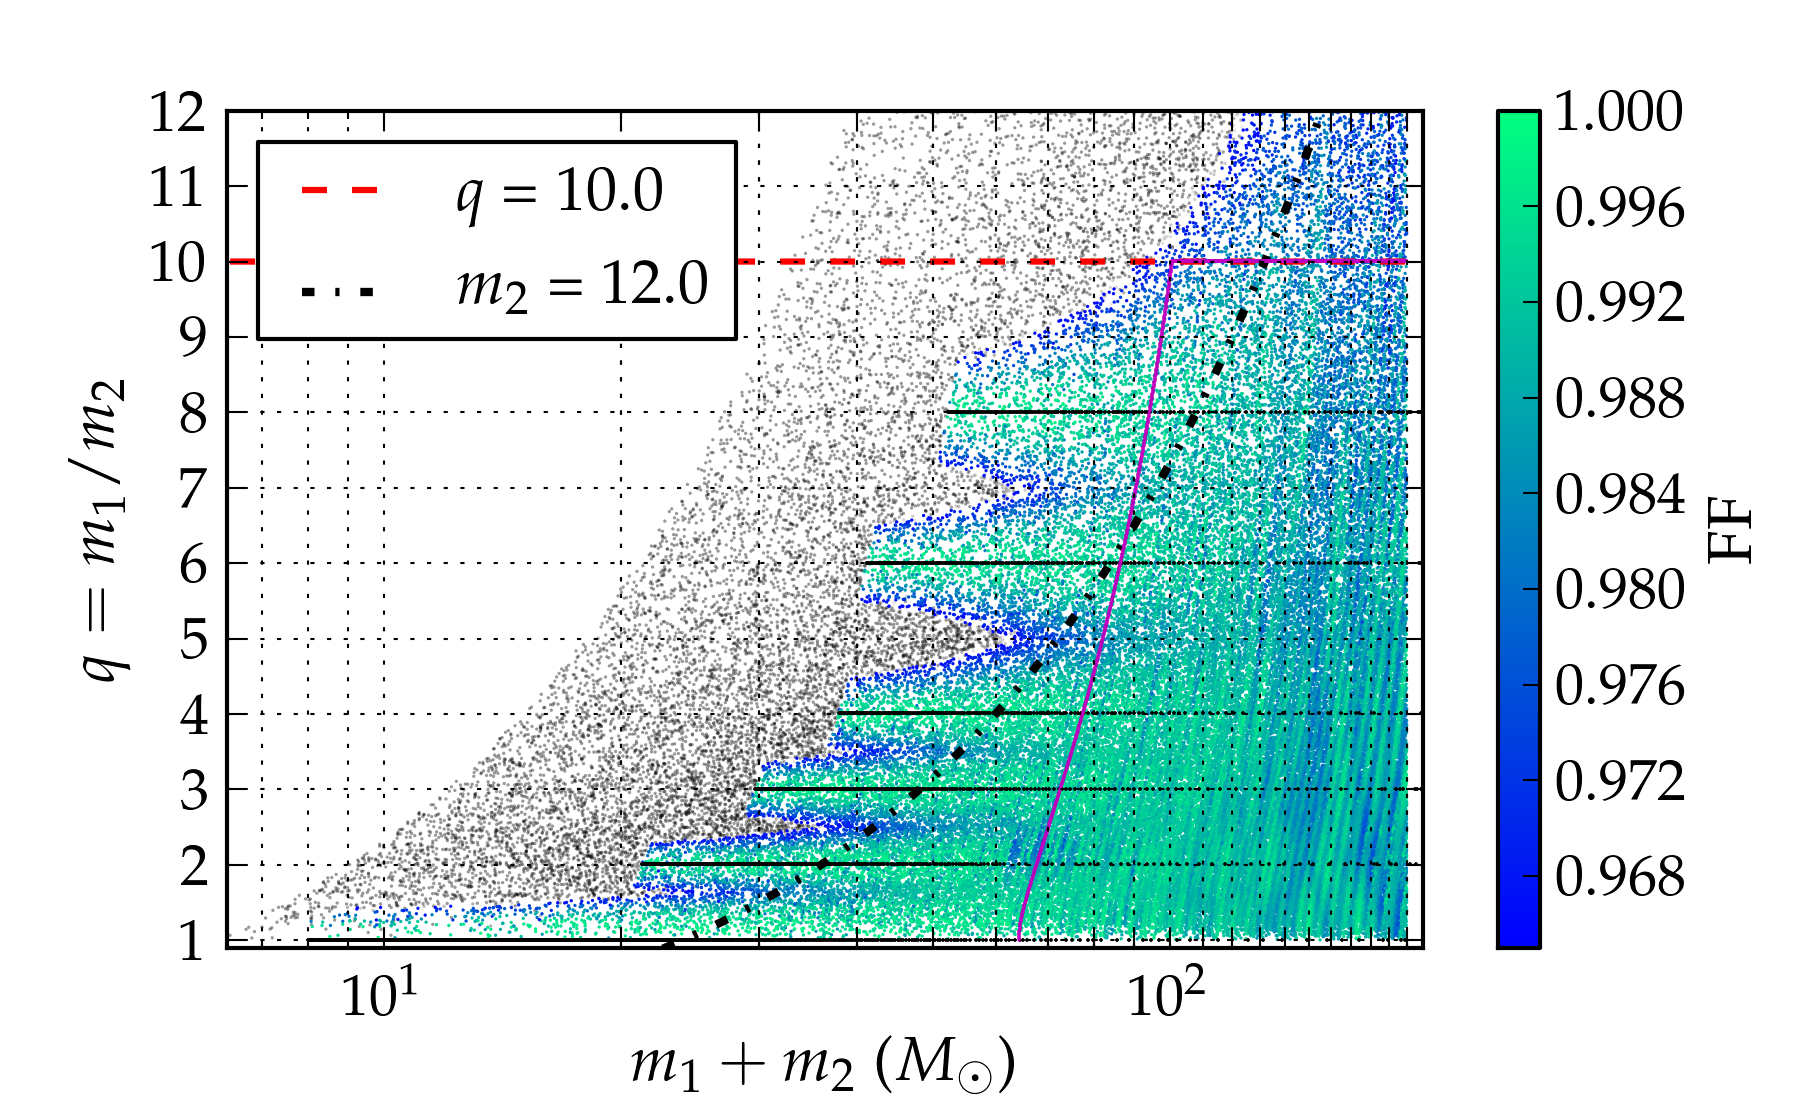
\includegraphics[width=\columnwidth]{bank001_lowM_01_stochastic_mtot200_logMq_NOhybMM.png}
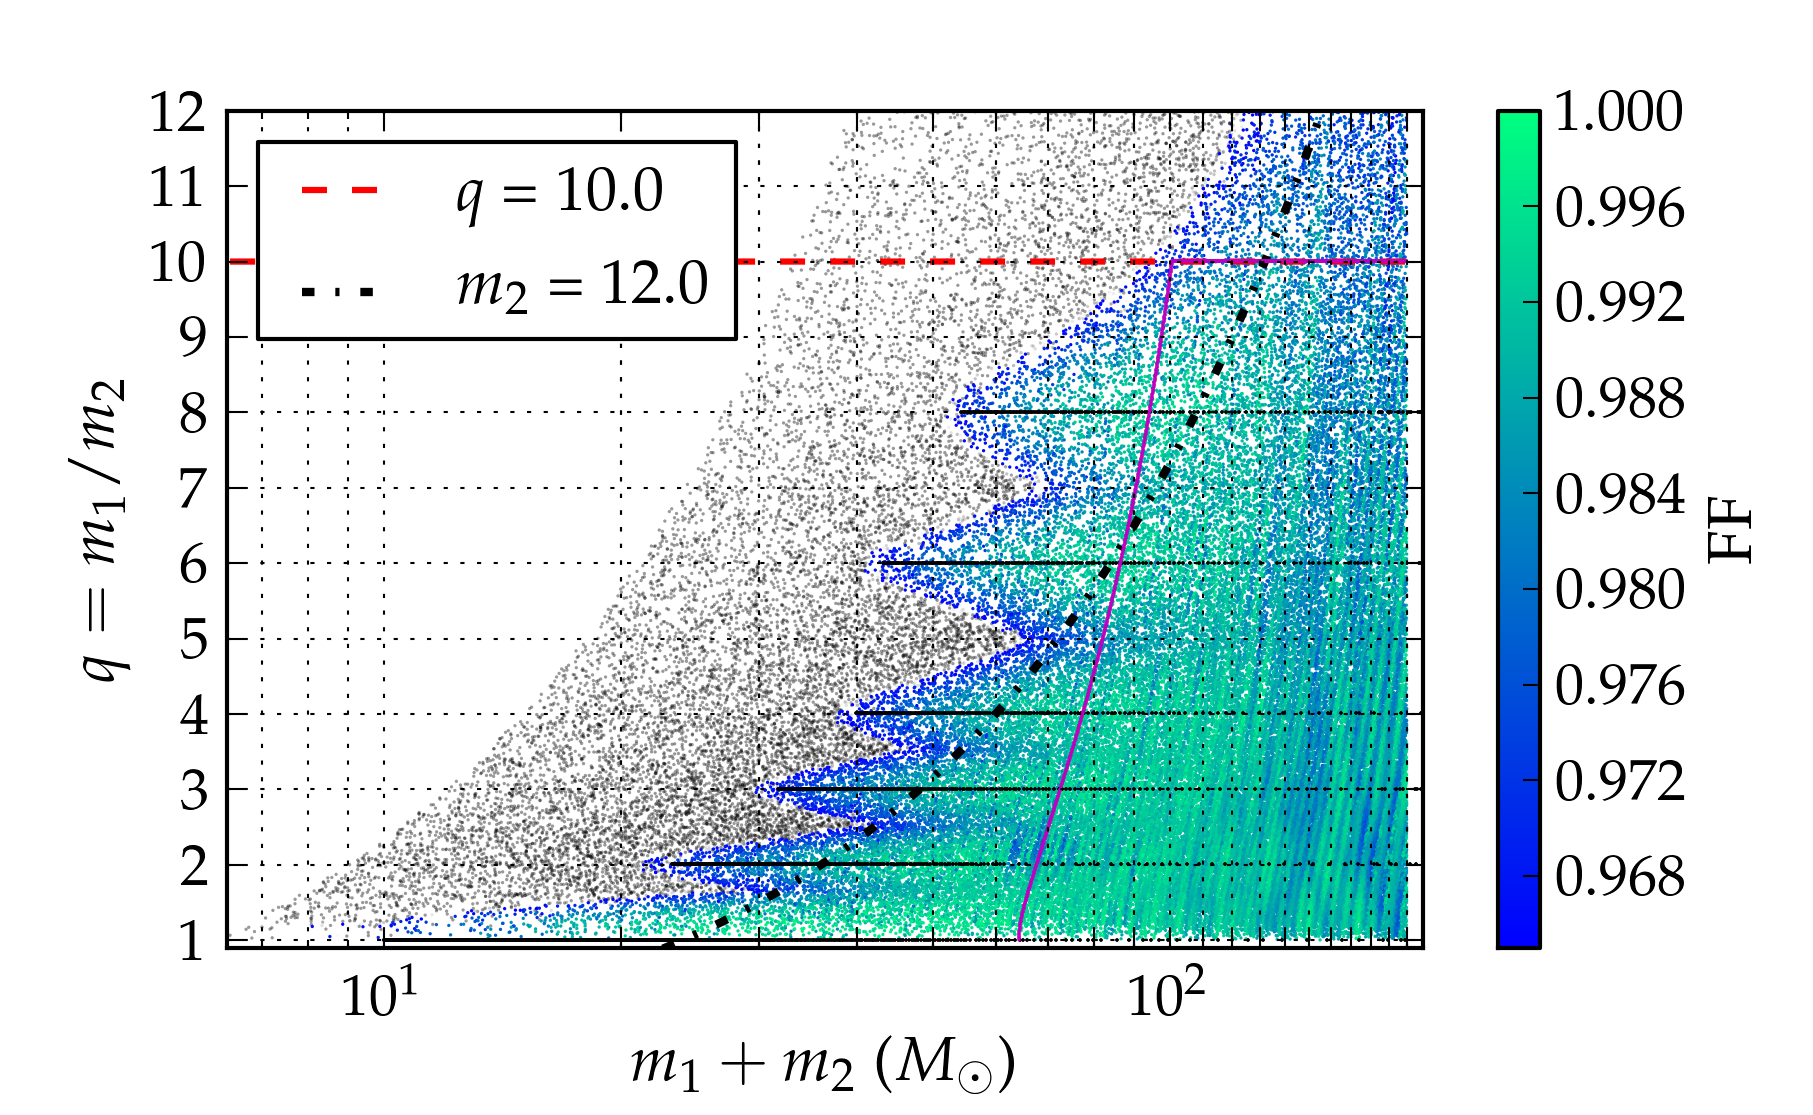
\includegraphics[width=\columnwidth]{bank001_lowM_01_stochastic_mtot200_logMq_hybMM.png}
\caption{\label{fig:Current-hybrids-stochastic-FF}These figures show fitting
  factors $\FF$ obtained when using a discrete mass-ratio template bank for
  $q=1,2,3,4,6,8$. For each mass-ratio, the templates are extended down 
  to a total mass where the NR-PN hybridization mismatch becomes
  $3\%$. The bank is placed using the stochastic algorithm, similar to 
  Ref.~\cite{Harry:2009ea,Ajith:2012mn,Manca:2009xw}. 
  The black dots show the location
  of the templates. The fitting factor on the left plot does 
  {\em not} take into account the hybridization error, and therefore shows the
  effect of the sparse placement of the templates alone. 
  The right plot accounts for the hybridization error
  and gives the actual fraction of the optimal SNR that would be recovered
  with this bank of NR-PN hybrid templates. The region bounded by the magenta 
  (solid) line in both plots indicates the lower end of the coverage of the 
  bank of un-hybridized NR waveforms. Lastly, the shaded grey dots show the 
  points where the fitting factor was below $96.5\%$.}
\end{center}
\end{figure*}
\begin{figure*}
\begin{center}
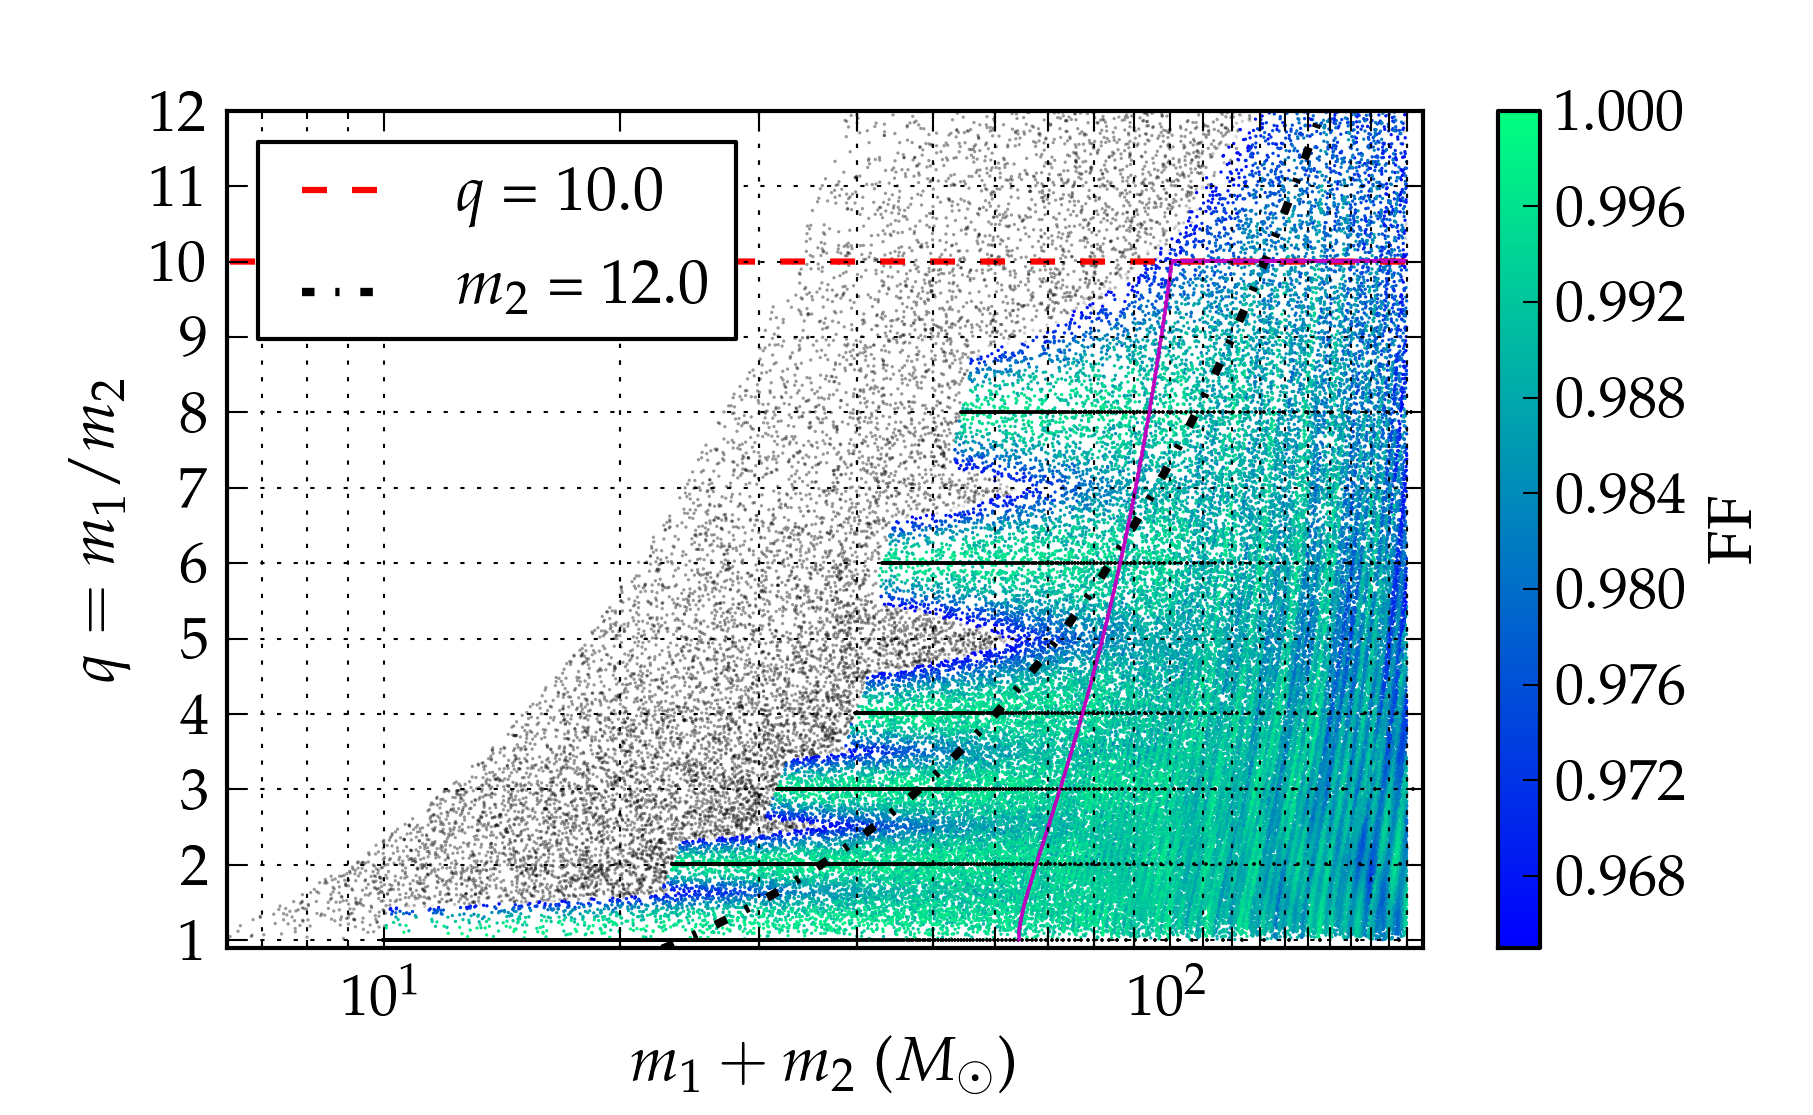
\includegraphics[width=\columnwidth]{bank_26022013_02_mtot200_logMq_NOhybMM.png}
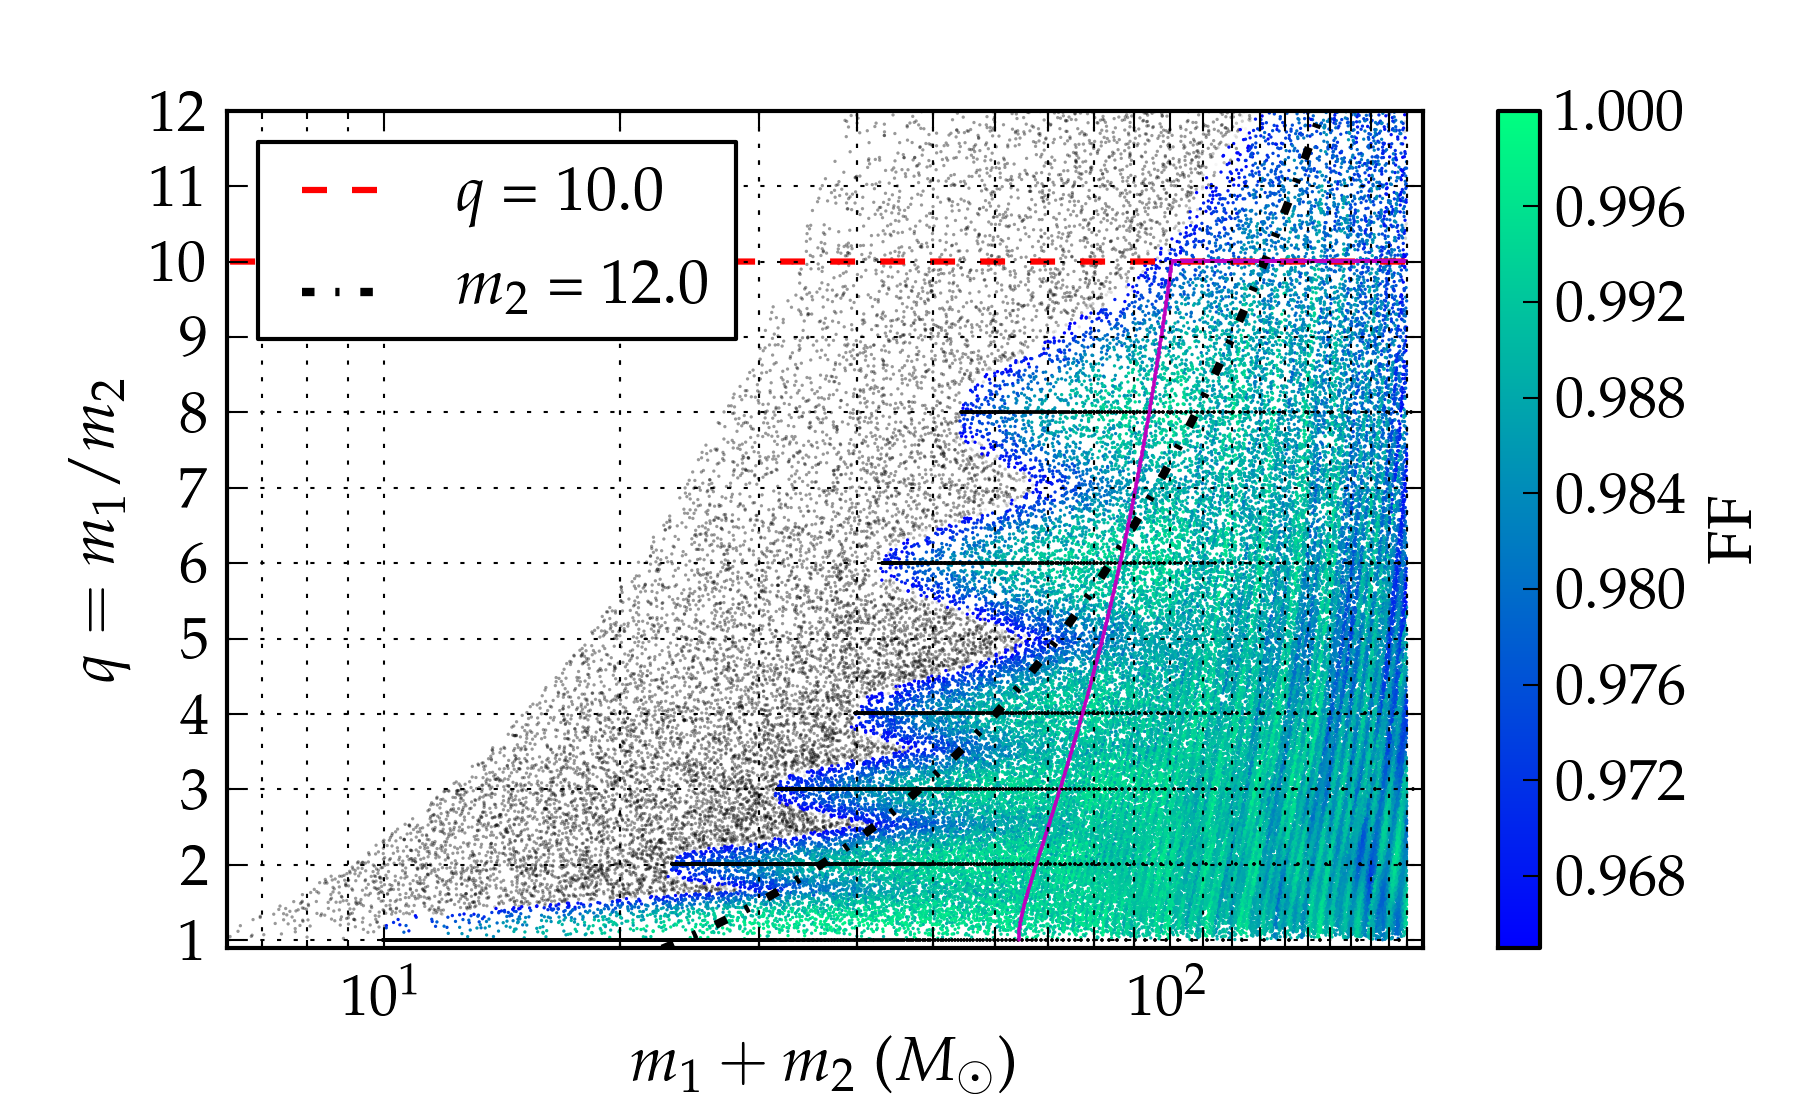
\includegraphics[width=\columnwidth]{bank_26022013_02_mtot200_logMq_hybMM.png}
\caption{\label{fig:Current-hybrids-FF}These figures are similar to 
  Fig.~\ref{fig:Current-hybrids-stochastic-FF}. The figures show fitting
  factors $\FF$ obtained when using a discrete mass-ratio template bank for
  $q=1,2,3,4,6,8$. For each mass-ratio, the templates are extended down 
  to a total mass where the NR-PN hybridization mismatch becomes
  $3\%$. Templates are placed independently for each mass-ratio, and span the 
  full range of total masses. For each mass-ratio, neighboring templates are 
  required to have an overlap of $97\%$. The union of the six single-$q$ 
  one-dimensional banks is taken as the final bank. The black dots show the 
  location of the templates. The fitting factor on the left plot does 
  {\em not} take into account the hybridization error, and therefore shows the
  effect of the sparse placement of the templates alone. The right plot accounts
  for the hybridization error
  and gives the actual fraction of the optimal SNR that would be recovered
  with this bank of NR-PN hybrid templates. The region bounded by the magenta 
  (solid) line in both plots indicates the lower end of the coverage of the 
  bank of un-hybridized NR waveforms. Lastly, the shaded grey dots show the 
  points where the fitting factor was below $96.5\%$.}
\end{center}
\end{figure*}

\begin{figure*}
\begin{center}
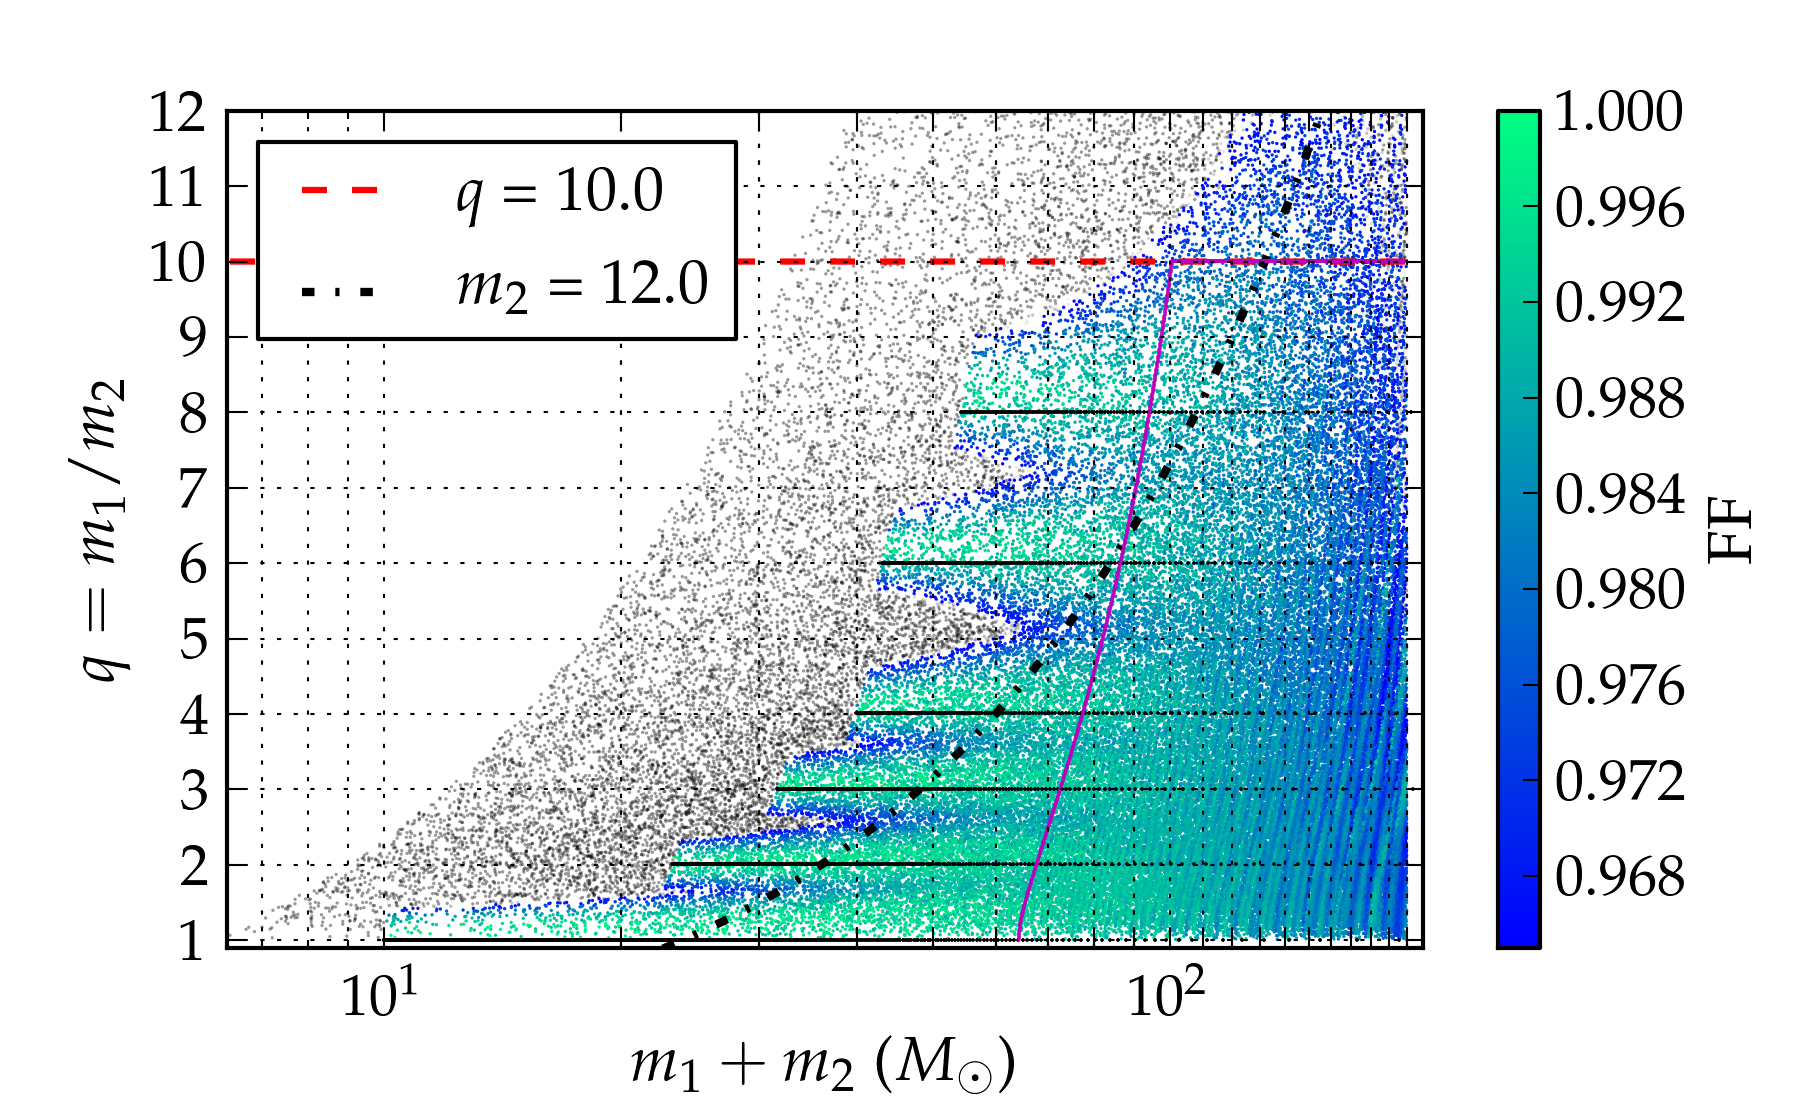
\includegraphics[width=\columnwidth]{bank_26022013_02_hybrids_mtot200_logMq_NOhybMM.png}
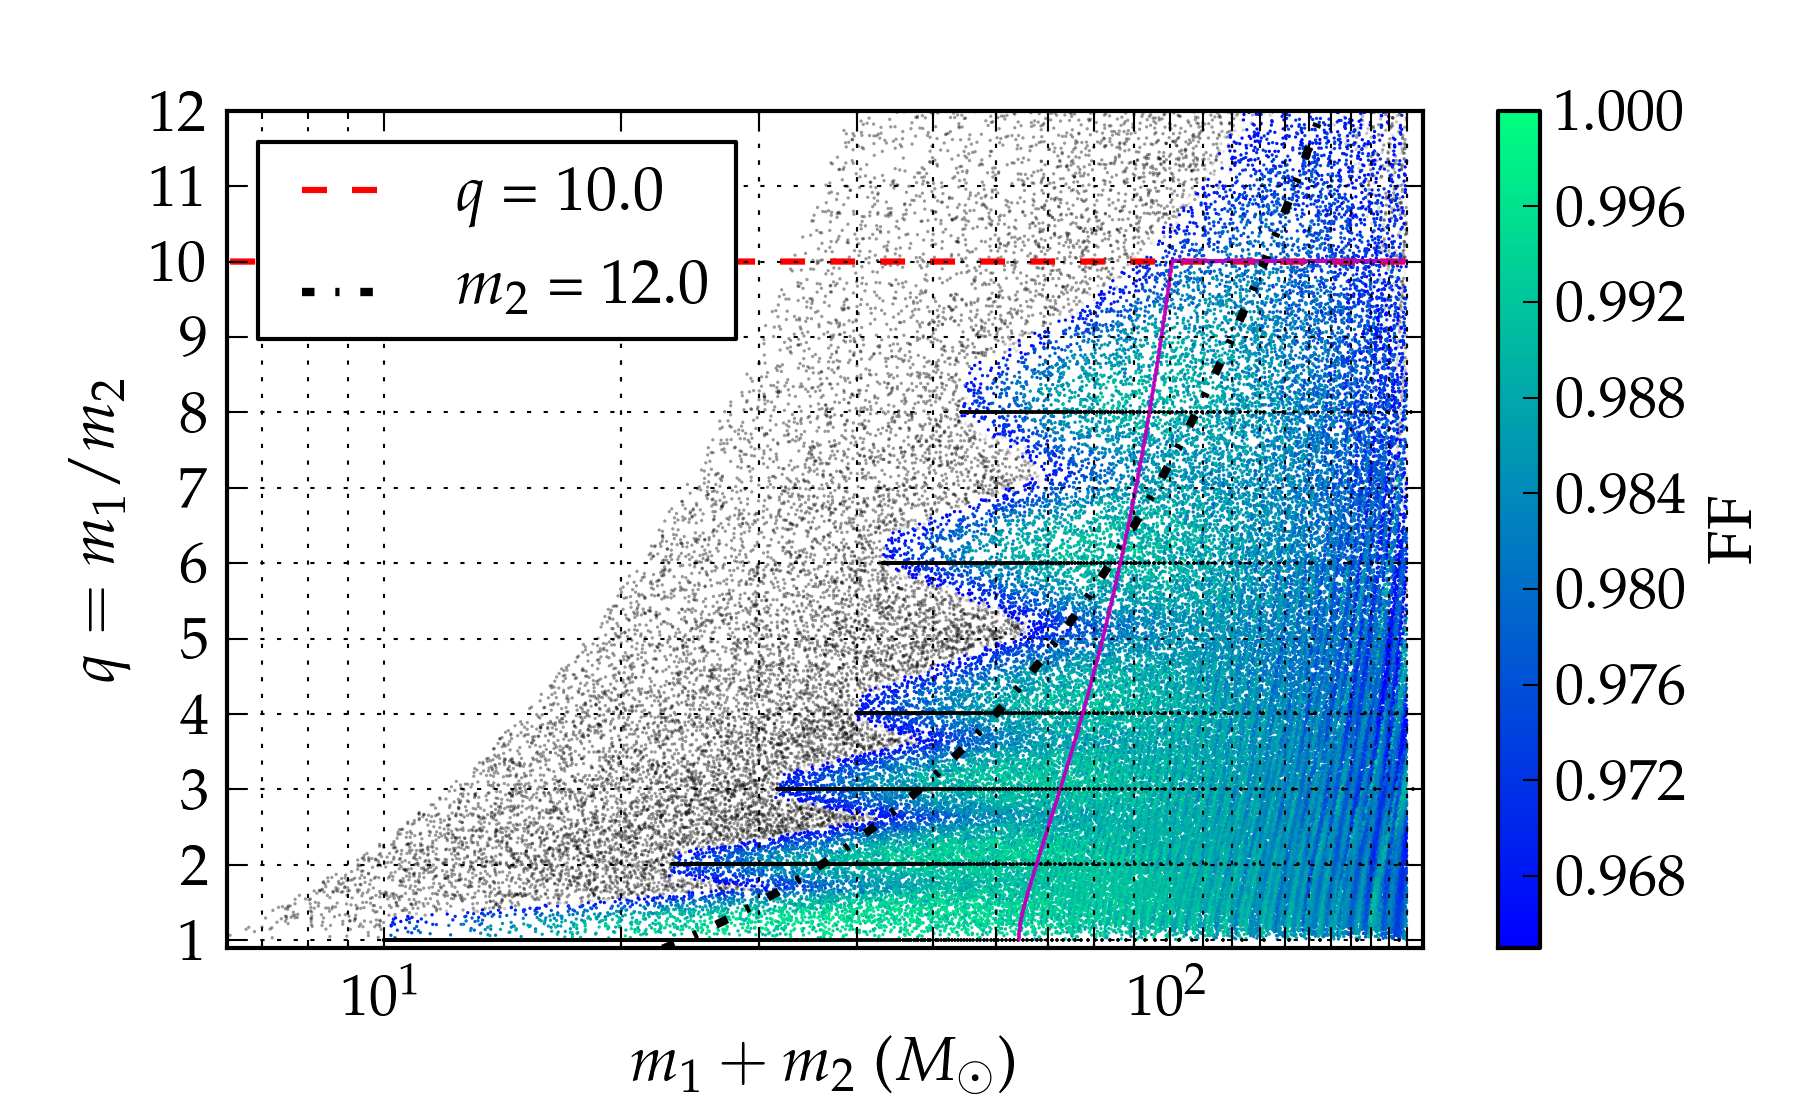
\includegraphics[width=\columnwidth]{bank_26022013_02_hybrids_mtot200_logMq_hybMM.png}
\caption{\label{fig:Current-real-hybrids-FF}This figure is similar to 
  Fig.~\ref{fig:Current-hybrids-FF}. The figures show fitting
  factors $\FF$ obtained when using a discrete mass-ratio template bank for
  $q=1,2,3,4,6,8$. Templates are placed independently for each mass-ratio, and 
  span the range of total masses, down to the region where the hybrid errors
  become $3\%$. For each mass-ratio, neighboring templates are 
  required to have an overlap of $97\%$. The union of the six single-$q$ 
  one-dimensional banks is taken as the final bank. The black dots show the 
  location of the templates. The GW signals are modeled using the EOBNRv2
  approximant~\cite{BuonannoEOBv2Main}, while TaylorT4+NR hybrids are used as
  templates. The fitting factor on the left plot shows the combined effect of 
  the sparse placement of the templates, and the (relatively small) 
  disagreement between the hybrid and EOBNRv2 waveforms. The right plot
  explicitly accounts for the hybridization error and gives the (conservative)
  actual fraction of the optimal SNR that would be recovered
  with this bank of NR-PN hybrid templates. The region bounded by the magenta 
  (solid) line in both plots indicates the lower end of the coverage of the 
  bank of un-hybridized NR waveforms. Lastly, the shaded grey dots show the 
  points where the fitting factor was below $96.5\%$.  }
\end{center}
\end{figure*}

%\textcolor{red}{How do we construct the stochastic bank, and how well does it perform?}\newline
We now consider template banks viable for hybrids constructed from currently 
available NR waveforms at mass ratios $q=1,2,3,4,6,8$. The lower mass limit,
in this case, is extended down to masses where the hybridization error 
exceeds $3\%$. We demonstrate two independent methods of laying
down the bank grid. First, we use the stochastic placement method that proceeds
as described in Sec.~\ref{s1:NRonlybank}. The templates are sampled over the
total mass - mass-rato $(M,q)$ coordinates, sampling $q$ from the restricted
set. The total mass $M$ is sampled from the continuous interval between the 
lower mass limit, which is different for each $q$, and the upper limit of
$200M_\odot$. To assess the SNR loss from the sparse placement
of the templates, we simulate a population of $100,000$ BBH signal waveforms,
with masses sampled with $3M_\odot\leq m_{1,2}\leq 200M_\odot$ and 
$M\leq 200M_\odot$, and filter them through the bank. This portion of the SNR
loss needs to be measured with both signals and templates in the same waveform
manifold. We use the EOBNRv2 approximant~\cite{BuonannoEOBv2Main} to model both, 
as it has been calibrated to most of the NR waveforms we consider here, and it
allows us to model waveforms for arbitrary systems. The left panel of
Fig.~\ref{fig:Current-hybrids-stochastic-FF} shows the
fraction of the optimal SNR that the bank recovers, accounting for its 
discreteness alone. We observe that, with just six mass-ratios, the bank 
can be extended to much lower masses before it is limited by the restricted
sampling of mass-ratios for the templates. For binaries with both black-holes 
more massive than $\sim 12M_\odot$, the spacing between mass-ratios was found 
to be sufficiently dense. The total SNR loss, after subtracting out 
the hybrid mismatches from Fig.~\ref{fig:Current-NR-PN-Errors}, are shown in 
the right panel of Fig.~\ref{fig:Current-hybrids-stochastic-FF}. 
At the lowest masses, the coverage shrinks between the lines of constant $q$ 
over which the templates are placed, due to the hybrid errors increasing 
sharply. We conclude that this bank is viable for hybrid templates for GW 
searches for BBHs with $m_{1,2}\geq 12M_\odot$, $1\leq q\leq 10$, and 
$M\leq 200M_\odot$. Over this region the bank will recover more than $96.5\%$
of the optimal SNR. This is a significant increase over the coverage allowed 
for with the purely-NR bank, the region of coverage of which is shown in the 
right panel of Fig.~\ref{fig:Current-hybrids-FF}, bounded at lowest masses by 
the magenta (solid) curve.


%\textcolor{red}{What is the second method, why do we use it, and how well does it compare?}\newline
Second, we demonstrate a non-stochastic algorithm of bank placement, with 
comparable results. We first construct six independent bank grids, each
restricted to one of the mass-ratios $q=1,2,3,4,6,8$, and spanning the full 
range of total masses. The spacing between neighboring templates is
given by requiring that the overlap between them be $97\%$. 
We take the union of these banks as the final 
two-dimensional bank. As before, we measure the SNR loss due to discreteness of
the bank and the waveform errors in the templates separately. To estimate the
former, we simulate a population of $100,000$ BBH systems, and filter
them through the bank. The signals and the templates are both modeled
with the EOBNRv2 model. The left panel of Fig.~\ref{fig:Current-hybrids-FF}
reveals the fraction of SNR recovered over the mass space, accounting for the 
sparsity of the bank alone, i.e. $1-\Gamma_\mathrm{bank}$. At lower masses, 
we again start to see gaps between the lines of constant mass ratio which become
significant at $m_{1,2} \leq 12M_\odot$. 
The right panel of Fig.~\ref{fig:Current-hybrids-FF} shows the final fraction 
of the optimal SNR recovered, i.e. the $\FF$ as defined in Eq.~(\ref{eq:FFGammas}). 
As before, these are computed by subtracting out the hybrid mismatches 
$\Gamma_\Hyb$ in addition to the discrete mismatches, as described in
Sec.~\ref{s1:quantifyingerrors}. 

The efficacy of both methods of template bank construction
can be compared from Fig.~\ref{fig:Current-hybrids-stochastic-FF} and 
Fig.~\ref{fig:Current-hybrids-FF}. We observe that the final banks from either
of the algorithms have very similar SNR recovery, and are both effectual over
the range of masses we consider here. Both were also found to give a very 
similar number of templates. The uniform-in-overlap method yields a grid 
with $2,325$ templates. The stochastic bank, on the other hand, was placed with a
requirement of $98\%$ minimal mismatch, and had $2,457$ templates. 
This however includes templates with $m_{1,2} < 12M_\odot$. Restricted
to provide coverage over the region with $m_{1,2}\geq 12M_\odot$, $1\leq q\leq 10$,
and $M\leq 200M_\odot$, the two methods yield banks with $627$ and $667$
templates respectively. The size of these banks is comparable to one 
constructed using the second-order post-Newtonian TaylorF2 hexagonal 
template placement method~\cite{SathyaBankPlacementTauN,BabaketalBankPlacement,
SathyaMetric2PN,Cokelaer:2007kx}, 
which yields a grid of $522$ and $736$ templates, for a minimal
match of $97\%$ and $98\%$, respectively.

%\textcolor{red}{How do we show the robustness of the banks using NR hybrids?}\newline
Finally, we test the robustness of these results using TaylorT4+NR hybrids 
as templates. As before, we simulate a population of $100,000$ BBH signal 
waveforms. As we do not have hybrids for arbitary binary
masses, we model the signals as EOBNRv2 waveforms. This population is filtered
against a bank of hybrid templates. The SNR recovered is shown in the left 
panel of Fig.~\ref{fig:Current-real-hybrids-FF}. Comparing with the left panels 
of Fig.~\ref{fig:Current-hybrids-stochastic-FF},~\ref{fig:Current-hybrids-FF}, 
we find that the EOBNRv2 manifold is a reasonable approximation for the hybrid 
manifold; and that, at lower masses, there is a small systematic bias in the 
hybrids towards EOBNRv2 signals with slightly higher mass-ratios.
The right panel of Fig.~\ref{fig:Current-real-hybrids-FF} 
shows the fraction of optimal SNR recovered after subtracting out the hybrid
mismatches from the left panel. The similarity of the $\FF$ distribution between 
the right panels of Fig.~\ref{fig:Current-real-hybrids-FF} and 
Fig.~\ref{fig:Current-hybrids-stochastic-FF},~\ref{fig:Current-hybrids-FF}
is remarkable. This gives us confidence that the EOBNRv2 model is a good 
approximation for testing NR/hybrid template banks, as we do in this paper; 
and that a template bank of NR+PN hybrids is indeed effectual for binaries 
with $m_{1,2}\geq 12M_\odot$, $M\leq 200M_\odot$ and $q\leq 10$.


